\documentclass[aspectratio=169]{beamer}
\setbeamertemplate{navigation symbols}{}
\usepackage{color,amsmath,comment, subfigure}
\usepackage{booktabs}
\usepackage{url}

%\setbeameroption{show notes}

%%%%%%%%%%%%%%%%%%%%%%%%%%
\title[]{Class 14: Strength of weak ties}
\author[]{Matthew J. Salganik}
\institute[]{Sociology 204: Social Networks\\Princeton University}
\date[]{
2/2 Weakness of weak ties
\vfill

\begin{flushleft}
\vspace{0.6in}

\includegraphics[width=0.1\textwidth]{figures/cc.png}
\end{flushleft}
}

\begin{document}
%%%%%%%%%%%%%%%%%%%%%%%%%%%
\frame{\titlepage}
%%%%%%%%%%%%%%%%%%%%%%%%%%%
\begin{frame}

\begin{figure}
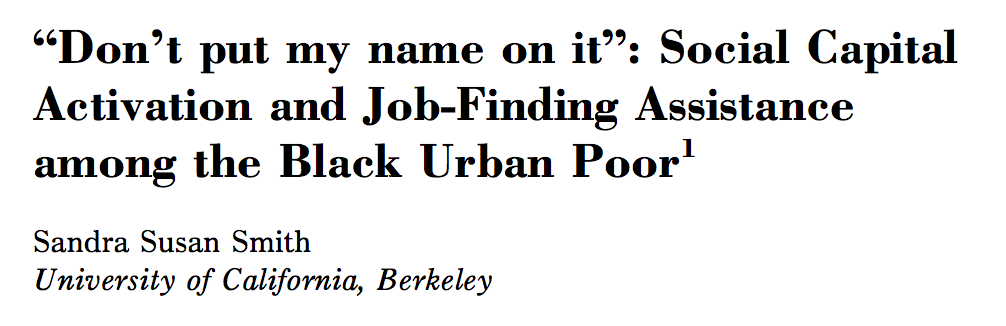
\includegraphics[width=0.7\textwidth]{figures/smith_dont_2005_title}
\end{figure}

\vfill
Paper has two main parts: theoretical and empirical.  For the theoretical part, this might remind you of reading Feld's paper on foci because you are entering into a long conversation.

\end{frame}
%%%%%%%%%%%%%%%%%%%%%%%%%%
\begin{frame}

What is social capital?
\pause
\begin{enumerate}
\item physical capital
\pause
\item human capital
\pause
\item social capital
\end{enumerate}

\pause
What is the most important kind of capital that get from Princeton?

\note {

POSSIBLE FOLLOW UP:
WOULD YOU RATHER COME TO PRINCETON FOR FOUR YEARS AND GET NO DIPLOMA OR GET A DIPLOMA AND NOT COME HERE AT ALL

}

\end{frame}
%%%%%%%%%%%%%%%%%%%%%%%%%%
\begin{frame}

Social capital from access to activation

\end{frame}
%%%%%%%%%%%%%%%%%%%%%%%%%%%%
\begin{frame}

``a baseline model of social capital activation (e.g., the probability that job seekers will receive job-finding assistance from job contacts with whom they are connected) would take into consideration properties of the:\\
\begin{itemize}
\item community
\item the network
\item the dyad
\item the individual''
\end{itemize}

\vfill
Note that Granovetter focused just on dyad

\end{frame}
%%%%%%%%%%%%%%%%%%%%%%%%%%%%
\begin{frame}

A bit more background about the network and community (individual and dyad are probably clear already).

\end{frame}
%%%%%%%%%%%%%%%%%%%%%%%%%%%
\begin{frame}

Idea about networks: Social capital is higher in networks with lots of social closure because of better information and more sanctioning.  

\begin{figure}
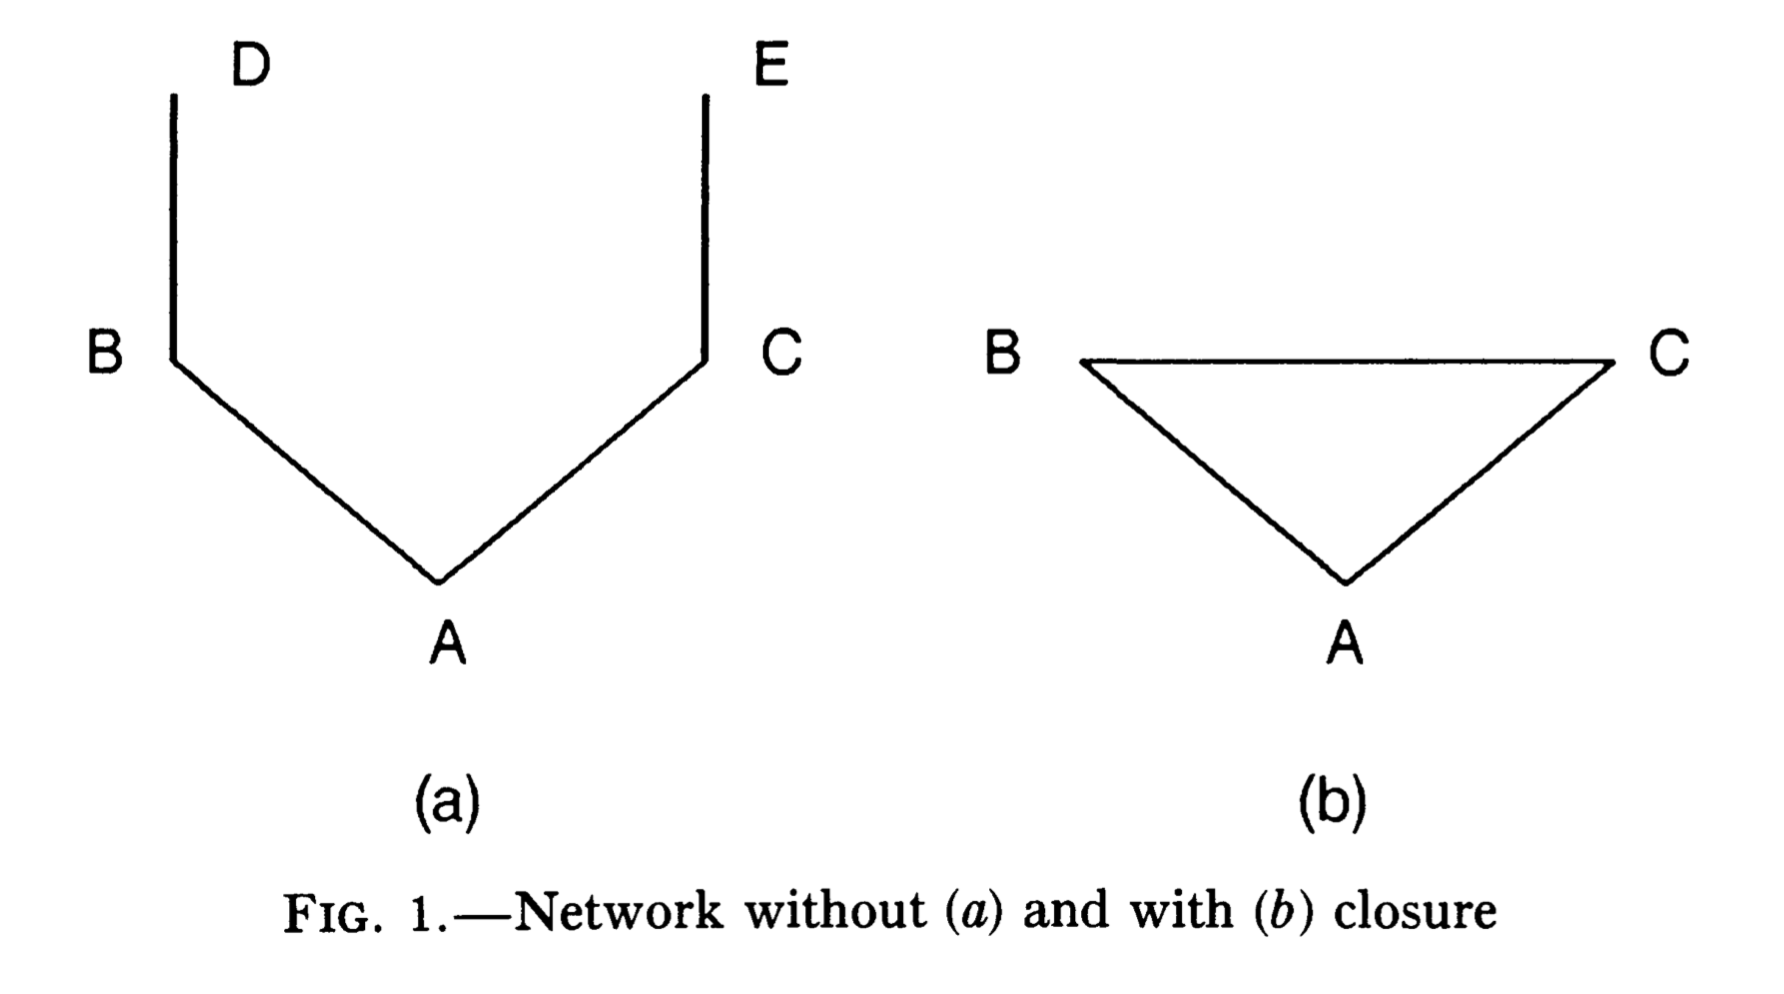
\includegraphics[width=0.7\textwidth]{figures/coleman_social_1988_fig1}
\end{figure}

More information: \url{https://www.jstor.org/stable/2780243}
\end{frame}
%%%%%%%%%%%%%%%%%%%%%%%%%%%
\begin{frame}

Idea about community: Concentrated disadvantage leads to generalized distrust.

\begin{figure}
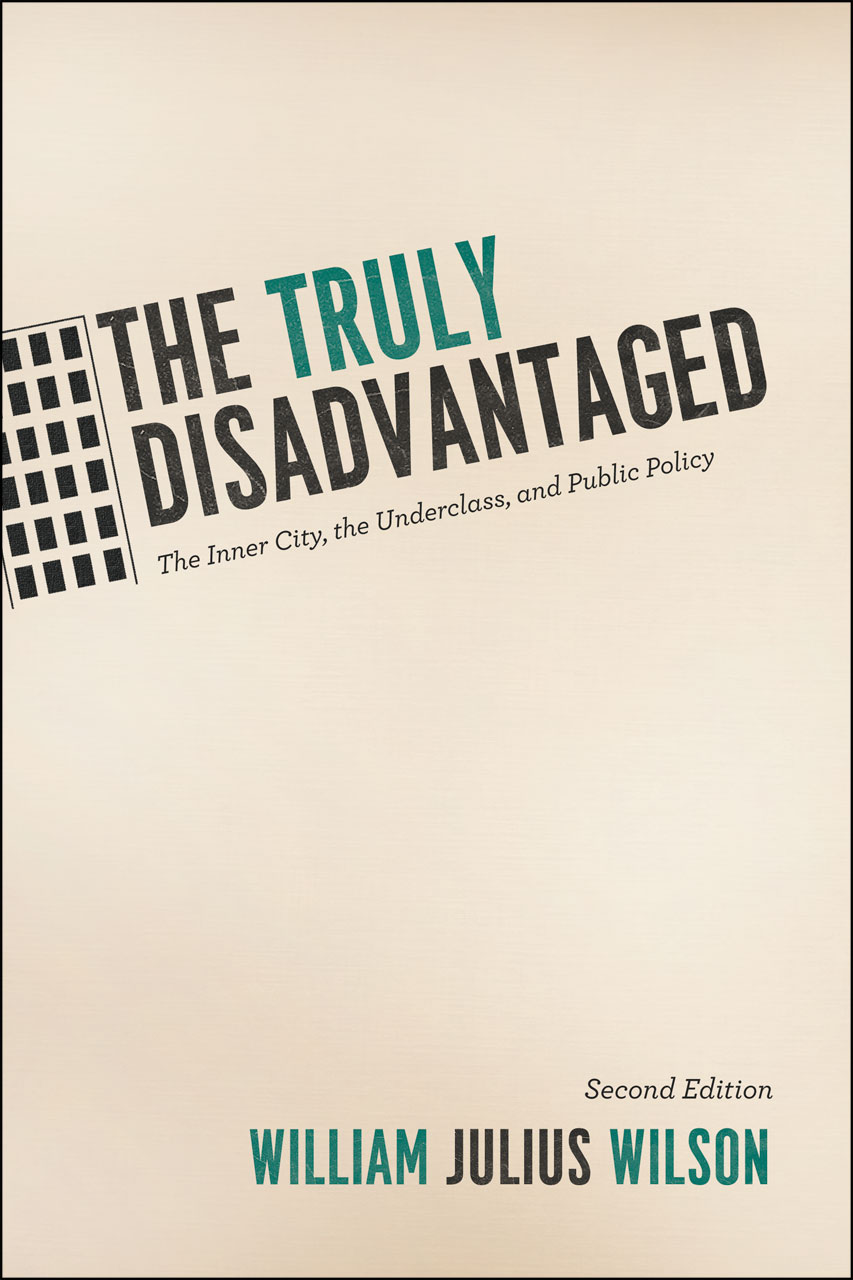
\includegraphics[height=0.7\textheight]{figures/wilson_truly_1987_cover}
\end{figure}

More information: \url{https://press.uchicago.edu/ucp/books/book/chicago/T/bo13375722.html}
\end{frame}
%%%%%%%%%%%%%%%%%%%%%%%%%%%
\begin{frame}

``a baseline model of social capital activation (e.g., the probability that job seekers will receive job-finding assistance from job contacts with whom they are connected) would take into consideration properties of the:\\
\begin{itemize}
\item community
\item the network
\item the dyad
\item the individual''
\end{itemize}

\vfill
Note that Granovetter focused just on dyad

\end{frame}
%%%%%%%%%%%%%%%%%%%%%%%%%%%%
\begin{frame}

Smith's two main questions:
\begin{enumerate}
\item When in possession of job information and/or influence, to what extent are the black urban poor willing to assist their job-seeking ties? \pause
\item Under what conditions are job contacts willing to extend job-finding assistance? Specifically, to what extent are decisions to assist affected by properties of the individual, the dyad, the network, and the community?
\end{enumerate}


\end{frame}
%%%%%%%%%%%%%%%%%%%%%%%%%%%%
\begin{frame}

\begin{itemize}
\item Main data: 105 in-depth interviews of low income African-Americans from 1 social service agency in Michigan in around 2000. \pause
\item Note the difference between in-depth interviews and surveys
\end{itemize}

\end{frame}
%%%%%%%%%%%%%%%%%%%%%%%%%%
\begin{frame}

Empirical findings \pause
\begin{itemize}
\item Many people are reluctant to provide help to job seekers, especially if they don't trust those job seekers and they themselves are in a precarious situation at their job \pause
\item People are more likely to help strong ties than weak ties, but they don't help all strong ties \pause
\item Offering assistance didn't seem to be related to social closure \pause
\item People in neighborhoods with concentrated disadvantaged were loss open to providing assistance (relative to those in low-moderate poverty neighborhoods)
\end{itemize}

\end{frame}
%%%%%%%%%%%%%%%%%%%%%%%
\begin{frame}

\begin{itemize}
\item ``accessed'' social capital is not the same as ``mobilized'' social capital.  Just knowing people who have access to job information is not enough. \pause
\item a weakness of weak ties
\end{itemize}

\note {
TIE BACK TO GRANOVETTER.  HOW DOES SMITH CHANGE HIS FINDINGS?
TIE BACK TO LEE SEARCH FOR AN ABORTIONIST, SOMETIMES STRONG TIES ARE MORE HELPFUL
}

\end{frame}
%%%%%%%%%%%%%%%%%%%%%%%%%%
\begin{frame}

A study in one social setting might produce a different result than a study in a different social setting.  Think back to cycles of length 4.  Not common in a high school in the US. More common in Likoma, Malawi.

\end{frame}
%%%%%%%%%%%%%%%%%%%%%%%%%%
\begin{frame}

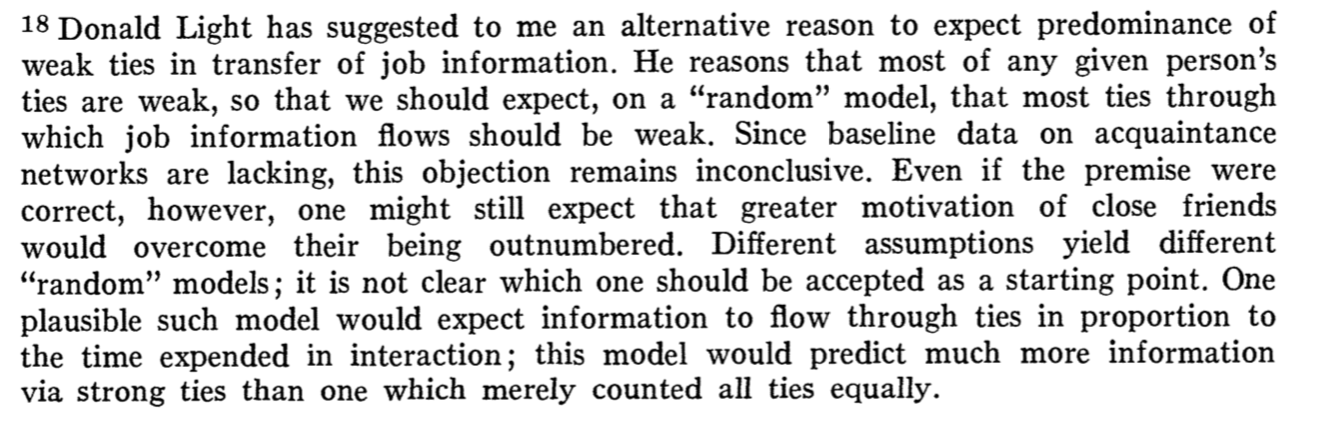
\includegraphics[width=\textwidth]{figures/granovetter_strength_1973_ft18}

\end{frame}
%%%%%%%%%%%%%%%%%%%%%%%%%%
\begin{frame}

Maybe people find jobs through weak ties because they have more weak ties?  

\pause

\vfill
\begin{figure}

\includegraphics[width=0.7\textwidth]{figures/yakubovich_weak_2005_title}
\end{figure}

\url{http://asr.sagepub.com/content/70/3/408.full.pdf+html}

Probability of finding a job through a weak tie is higher than finding a job through a strong tie (in Samara, Russia in 1998)

\end{frame}
%%%%%%%%%%%%%%%%%%%%%%%%%%
\begin{frame}

Summary:
\begin{itemize}
\item your weak ties might be your most important, but only if they are bridging 
\pause
\item weak ties also help hold communities together
\pause
\item ties alone might be enough if they can't be activated
\pause
\item activation of ties depends on the person, the dyad, the network, and the community
\end{itemize}


\end{frame}
%%%%%%%%%%%%%%%%%%%%%%%%%%
\begin{frame}

\begin{itemize}
\item Gladwell, M. (2010). Small change: The revolution will not be tweeted. \textit{New Yorker}.
\item Centola, D. and Macy, M.W. (2007). Complex contagion and the weakness of long ties. \textit{American Journal of Sociology}.
\item Centola, D. (2010). The spread of behavior in an online social network experiment. \textit{Science}.
\end{itemize}

\end{frame}
%%%%%%%%%%%%%%%%%%%%%%%%%%

\end{document}
